\chapter{Kiến thức nền tảng}
\label{Chapter2}

\noindent \textit{Trong chương này, đầu tiên nhóm chúng em trình bày về thuật toán ``Matrix factorization'' - thuật toán đề xuất sản phẩm bằng cách phân rã ma trận tương tác. Sau đó nhóm chúng em sẽ trình bày về thuật toán ``Gradient descent'' - thuật toán mà nhóm chúng em sẽ sử dụng để cực tiểu hóa hàm chi phí của  ``Matrix factorization''. Ngoài ra, nhóm chúng em còn trình bày về ``Naive bayes'' và ``Logistic regression'' - hai mô hình phân lớp mà nhóm chúng em sẽ sử dụng để ước lượng propensity trong IPS. Chương này, đặc biệt là về phần ``Matrix factorization'' cung cấp những kiến thức nền tảng để có thể hiểu rõ về những cải tiến mà nhóm em tìm hiểu ở chương kế tiếp.}

\section{``Matrix factorization''}
\label{section:MF}
``Matrix factorization'' là một phương pháp thuộc nhóm lọc cộng tác (collaborative filtering), một nhóm các phương pháp tập trung vào mối quan hệ giữa các người dùng, dựa trên đánh giá của các người dùng trước đó trong hệ thống. Các phương pháp lọc cộng tác này sẽ dựa trên ý tưởng những người dùng có cùng sở thích đối với một số sản phẩm nhất định, thì cũng có cùng sở thích đối với sản phẩm khác; do đó nó sẽ đề xuất sản phẩm cho người dùng dựa trên các sản phẩm mà người dùng giống với họ đã thích.

\subsection{Hàm dự đoán của ``Matrix factorization''}
Phương pháp ``Matrix factorization'' sẽ phân tích ma trận tương tác của người dùng và sản phẩm $Y$ thành tích của hai ma trận $V$ và $W$, sao cho từ hai ma trận $V$ và $W$ này ta có thể xây dựng lại được ma trận $Y$ càng chính xác càng tốt. Một cách cụ thể, ma trận tương tác dự đoán được của ta có thể ước lượng như sau (hình \ref{fig:chap2_MF1} minh họa phương pháp ``Matrix factorization''):
\begin{equation}
\label{eq:2.1_MF}
    Y \approx \hat{Y} = V \times W^T
\end{equation}

\begin{figure}[h]
    \centering
    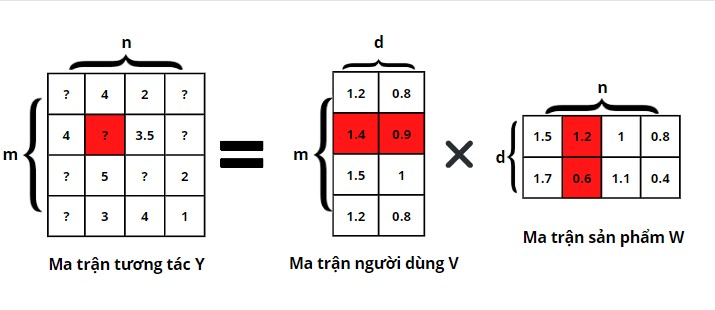
\includegraphics[width = \textwidth]{images/Chapter2/MF1.jpg}
    \caption{Matrix Factorization. Ma trận tương tác $Y$ sẽ được phân rã thành ma trận đại diện cho người dùng $V$ và đại diện cho sản phẩm $W$.}
    \label{fig:chap2_MF1}
\end{figure}
Trong đó:
\begin{itemize}
    \item Ma trận tương tác $Y$ là ma trận thưa có kích thước là $m \times n$ tương ứng với m người dùng đánh giá cho n sản phẩm. Ma trận $\hat{Y}$ là ma trận dự đoán có cùng kích thước với $Y$.
    \item $d$ là hyperparameter được điều chỉnh trong quá trình huấn luyện mô hình, đại diện cho số lượng các đặc trưng tiềm ẩn. Các đặc trưng tiềm ẩn mô tả sự liên quan giữa các người dùng và các sản phẩm. Ví dụ như trong hệ thống đề xuất phim, các đặc trưng tiềm ẩn có thể là thể loại, ngôn ngữ, diễn viên hay bất kì các đặc trưng nào khác; hoặc có thể là bất cứ sự liên quan khác giữa người dùng và sản phẩm mà ta không cần đặt tên cụ thể.
    \item Ma trận $V$ có kích thước $m \times d$ và là ma trận đại diện cho người dùng. Trong ma trận này, người dùng thứ $u$ sẽ tương ứng với hàng thứ $u$ trong ma trận và sẽ được kí hiệu là $v_u$. Các hệ số trong véc-tơ $v_u$ sẽ đo lường mức độ yêu thích của người dùng $u$ cho các đặc trưng ẩn, hệ số càng cao tương ứng với người dùng $u$ càng thích các sản phẩm mang đặc trưng đó.
 
    \item Tương tự, ma trận $W$ có kích thước $d \times n$ và là ma trận đại diện cho sản phẩm. Trong ma trận này, sản phẩm thứ $i$ sẽ tương ứng với hàng thứ $i$ trong ma trận và sẽ được kí hiệu là $w_i$. Các hệ số trong véc-tơ $w_i$ sẽ đo lường mức độ sản phẩm $i$ mang các đặc trưng ẩn, hệ số càng cao tương ứng với sản phẩm $i$ mang đặc trưng đó càng lớn.
\end{itemize}
Mục tiêu của chúng ta là đề xuất cho người dùng $u$ các sản phẩm $i$ mang đặc trưng mà người dùng $u$ thích, tương ứng với giá trị của $v_u$ và $w_i$ đều cao dẫn đến giá trị của $v_u^T\times w_{i}$ càng cao. Khi đó, đánh giá của người dùng $u$ cho sản phẩm $i$ sẽ được tính toán bằng tích của 2 véc-tơ $v_u$ và $w_i$. Cụ thể như công thức sau:
\begin{equation}
\label{eq:2.1_yui_nonbias}
    \hat{Y}_{u,i} = v_{u} \times w_i^T
\end{equation}

Trong thực tế, một số người dùng sẽ có thiên hướng đánh giá cao hơn các người dùng khác, hay một số sản phẩm sẽ bị đánh giá thấp hơn trung bình. Do đó đánh giá của người dùng $u$ cho sản phẩm $i$ cần cộng thêm các offset cho riêng từng người dùng $a_u$ từng sản phẩm $b_i$ và giá trị trung bình cho toàn bộ đánh giá $c$. Khi đó công thức \ref{eq:2.1_yui_nonbias} được viết lại như sau:
\begin{equation}
\label{eq:2.1_yui_bias}
    \hat{Y}_{u,i} = v_{u}\times w_i^{T} + a_u + b_i + c
\end{equation}
\subsection{Tìm các tham số của hàm dự đoán của ``Matrix Factorization''}
Mục tiêu chính của việc huấn luyện mô hình ``Matrix Factorization'' là tìm giá trị của hai ma trận $V$ và $W$. Vì vậy hai ma trận này sẽ được ước lượng bằng cách cực tiểu hóa trung bình bình phương sai số giữa đánh giá dự đoán và đánh giá thực trên các đánh giá quan sát được. Với $A$ là ma trận chứa các offset, hàm mục tiêu được định nghĩa cụ thể như sau:
\begin{equation}
\label{eq:2.1_objective}
    \operatorname*{argmin}_{V,W,A} \sum_{(u,i)\in\kappa} (Y_{u,i} - \hat{Y}_{u,i})^2 + \lambda(||V||_{F}^2 + ||W||_{F}^2+A)
\end{equation}
Ở đây: 
\begin{itemize}
    \item $\kappa$ là tập dữ liệu chứa các đánh giá quan sát được.
    \item $\lambda$ là tham số regularization $(0 \leq \lambda \leq 1)$ và $\lambda(||V||_{F}^2 + ||W||_{F}^2)$ là regularization để tránh hiện tượng overfitting của mô hình.
    \item $||\cdot||_{F}$ là ký hiệu của chuẩn Frobenius, bằng căn bậc hai của tổng bình phương tất cả các phần tử của ma trận.
\end{itemize}

Để cực tiểu hóa hàm mục tiêu này, ta có thể sử dụng thuật toán ``Gradient Descent'' sẽ được trình bày ở phần \ref{section:Gradientdescent}.

\section{``Logistic regression''}
``Logistic regression'' là một mô hình học có giám sát và được sử dụng trong bài toán phân lớp nhị phân. Mô hình này hoạt động bằng cách sử dụng hàm ``sigmoid'' để phân lớp các véc-tơ đầu vào. Trong khóa luận của nhóm chúng em, ``Logistic regression'' được sử dụng để ước lượng propensity (tiền đề cho việc tính toán độ đo IPS) thông qua các thuộc tính đặc trưng của người dùng và sản phẩm.

\subsection{Hàm ``sigmoid''}
Hàm ``sigmoid'' là một hàm số liên tục có đạo hàm không âm tại mọi điểm. Hàm ``sigmoid'' sẽ ánh xạ tất cả số thực vào khoảng (0,1), điều này làm cho nó trở thành một hàm phù hợp cho bài toán phân lớp. Hình \ref{fig:2.2_sigmoid} minh họa đồ thị hàm số ``sigmoid''. Thông qua đồ thị ta có thể thấy khi đầu vào càng tiến đến $+\infty$ giá trị khi đi qua hàm ``sigmoid'' càng tiến gần 1, ngược lại, khi đầu vào càng tiến đến $-\infty$ giá trị khi đi qua hàm ``sigmoid'' càng tiến gần về 0.
\begin{figure}[h]
    \centering
    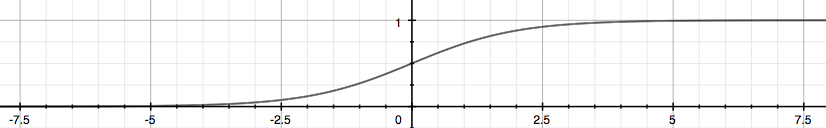
\includegraphics[width=\textwidth, height=5cm]{images/Chapter2/sigmoid.png}
    \caption{Đồ thị hàm số số ``Sigmoid'' (hình vẽ được lấy từ bài giảng của GS. Andrew Ng trong khóa học "Machine Learning" ở trang \href{https://www.coursera.org/learn/machine-learning}{coursera.org}).}
    \label{fig:2.2_sigmoid}
\end{figure}

Hàm ``sigmoid'' sẽ được tính toán thông qua công thức:
\begin{equation}
    \sigma(x) = \frac{1}{1+ e^{x}}
    \label{eq:2.2_sigmoid}
\end{equation}

\subsection{Hàm dự đoán của ``Logistic regression''}
Với một véc-tơ đầu vào $x \in \mathbb{R}^{D\times 1}$, với $D$ là số lượng đặc trưng của véc-tơ đầu vào, hàm dự đoán $h(x)$ của ``Logistic regression'' sẽ trả về một giá trị nằm trong khoảng $(0,1)$. Giá trị trả về này cho biết xác suất $p(y=1|x)$, với $y$ là đầu ra của véc-tơ đầu vào $x$. Khi đó, xác suất đầu ra $y$ là 0 sẽ được tính toán bằng [$p(y=0|x) = 1 - p(y=1|x)$]. Như vậy, ta có thể biết được véc-tơ đầu vào $x$ thuộc lớp nào dựa trên một một ngưỡng bằng 0.5, tức là $h(x) \geq 0.5$ thì véc-tơ đầu vào $x$ thuộc lớp 1 và ngược lại $h(x) \leq 0.5$ thì véc-tơ đầu vào $x$ sẽ thuộc lớp 0.

Cụ thể, hàm dự đoán h(x) của ``Logistic regression'' như sau:
\begin{equation}\label{eq:2.2_hx}
    \begin{split}
        h(x) &= p(y=1|x)\\
        &= \sigma(W^T x)\\
        &= \frac{1}{1+ e^{W^T x}}
    \end{split}
\end{equation}
với $W$ là các tham số của hàm dự đoán.


\subsection{Tìm các tham số của hàm dự đoán của ``Logistic regression''}
\subsubsection{Xác suất $p(y|x)$}
Mục đích của chúng ta là tìm các tham số của hàm dự đoán $W$ sao cho $h(x)$ càng gần với 1 càng tốt đối với các điểm dữ liệu thuộc lớp 1 và càng gần với 0 với các điểm dữ liệu thuộc lớp 0. Như đã đề cập ở trước:
\begin{align}
    p(y=1|x) &= \sigma(W^T x) \label{eq:2.2_y1}\\
    p(y=0|x) &= 1 - \sigma(W^T x)\label{eq:2.2_y2}
\end{align}

Đặt giá trị dự đoán của mô hình là $\alpha = \sigma(W^T x)$, theo phân phối Bernoulli ta gộp 2 phương trình \ref{eq:2.2_y1} và \ref{eq:2.2_y2} lại thành:
\begin{equation}
    p(y|x) = \alpha^y(1-\alpha)^{1-y}
    \label{eq:2.2_alpha}
\end{equation}
\subsubsection{Tìm tham số W}
Cho tập huấn luyện ${ (x^{(1)}, y^{(1)}), \dots, (x^{(N)}, y^{(N)}) ) }$, với $N$ là số lượng các véc-tơ đầu vào. Để tìm ra được tham số $W$ của hàm dự đoán của ``Logistic regression'' ở công thức \ref{eq:2.2_hx}, ta sẽ dùng phương pháp ``maximum likelihood''. Với giả định các mẫu dữ liệu trong tập huấn luyện được phát sinh một cách độc lập, ta có hàm ``likelihood'' sau:

\begin{equation}\label{eq:2.2_L}
    \begin{split}
        L(W) &= p(Y|X)\\
        &= \prod_{i=1}^{N} p(y^{(i)}|x^{(i)})\\
        &= \prod_{i=1}^{N} (\alpha^{(i)})^{y^i}(1-(\alpha^{(i)}))^{1-y^i}
    \end{split}
\end{equation}

Trong đó:
\begin{itemize}
    \item $X = \{x^{(1)}, \dots, x^{(N)} \}$ và $Y = \{y^{(1)}, \dots, y^{(N)} \}$.
\end{itemize}

Ta tìm $W$ sao cho hàm ``likelihood'' $L(W)$ đạt cực đại. Cực đại $L(W)$ tương đương với cực tiểu hàm ``negative log-likelihood'' $-log(W)$.

Như vậy, ta sẽ tìm các tham số $W$ của hàm dự đoán của ``Logistic regression'' sao cho hàm chi phí sau đạt cực tiểu:
\begin{equation}\label{eq:2.2_C}
    \begin{split}
        C(W) &= -log(L(W))\\
        &= - \sum_{i=1}^{N} (y^{i} log(\alpha^{(i)}) + (1-y^{i})log(1-\alpha^{(i)}))
    \end{split}
\end{equation}


Để cực tiểu hàm này, ta có thể sử dụng thuật toán ``Gradient Descent'' (sẽ được trình bày ở các phần sau).
\section{``Naive bayes''}
``Naive bayes'' là một mô hình học có giám sát và thường được sử dụng trong bài toán phân lớp. Mô hình này hoạt động bằng cách sử dụng định lý ``Bayes'' để phân lớp các véc-tơ đầu vào, tuân theo một giả định là các biến đầu vào độc lập với nhau. Trong khóa luận của nhóm chúng em, ``Naive bayes'' được sử dụng để ước lượng propensity bằng cách sử dụng ma trận tương tác và một phần nhỏ dữ liệu kiểm tra tuân theo phân phối đều.
\subsection{Định lý ``Bayes''}
Định lý ``Bayes'' là một định lý về xác suất có điều kiện. Nó được sử dụng để tính toán xác suất một biến cố $A$ xảy ra khi biết biến cố $B$ xảy ra, được tính toán thông qua công thức sau:
\begin{equation}
    p(A|B) = \frac{p(B|A)p(A)}{p(B)}
    \label{eq:2.3_bayes}
\end{equation}
Trong đó:
\begin{itemize}
    \item $p(A|B)$ là xác suất biến cố $A$ xảy ra với điều kiện biến cố $B$ xảy ra. Tương tự, $p(B|A)$ là xác suất biến cố $B$ xảy ra với điều kiện biến cố $A$ xảy ra.
    \item $p(A)$ và $p(B)$ là xác suất xảy ra 2 biến cố $A$ và $B$ độc lập, không bị tác động bởi biến cố khác.
\end{itemize}
\subsection{Hàm dự đoán của ``Naive bayes''}
Với một véc-tơ đầu vào $x \in \mathbb{R}^{D\times 1}$, với $D$ là số lượng đặc trưng của véc-tơ đầu vào, hàm dự đoán $h(x)$ của ``Naive Bayes'' sẽ trả về một véc-tơ gồm có $K$ phần tử (ứng với $K$ lớp), trong đó phần tử thứ $k$ cho biết xác suất $p(y=k|x)$ với $y \in \{1,2,\dots,K\}$ là nhãn lớp của véc-tơ đầu vào $x$. Như vậy, véc-tơ đầu vào $x$ sẽ thuộc lớp có xác suất lớn nhất.
\begin{equation}\label{eq:2.3_hx}
    \begin{split}
        h(x) &= 
        \begin{bmatrix}
            p(y=1|x)\\
            p(y=2|x)\\
            \vdots\\
            p(y=k|x)
        \end{bmatrix}\\
        &= 
        \begin{bmatrix}
            \frac{p(x|y=1)p(y=1)}{p(x))}\\
            \frac{p(x|y=2)p(y=2)}{p(x)}\\
            \vdots\\
            \frac{p(x|y=k)p(y=k)}{p(x))}
        \end{bmatrix}\\
        &=
        \begin{bmatrix}
            p(x|y=1)p(y=1)\\
            p(x|y=2)p(y=2)\\
            \vdots\\
            p(x|y=k)p(y=k)
        \end{bmatrix}
    \end{split}
\end{equation}
Trong đó:
\begin{itemize}
    \item $p(y=k)$ là xác suất thuộc lớp $k$.
    \item $p(x|y=k)$ là xác suất véc-tơ đầu vào $x$ thuộc lớp $k$.
\end{itemize}

\subsection{Tìm các xác suất của hàm dự đoán của ``Naive Bayes''}
\subsubsection{Xác suất p(y)}
Gọi $N$ là số lượng các mẫu huấn luyện, $N_k$ ($k \in {1,2,\dots,K}$) là số lượng các véc-tơ đầu vào thuộc lớp $k$. Xác suất $p(y=k)$ có thể được tính toàn bằng số điểm dữ liệu trong tập huấn luyện thuộc lớp này chia cho tổng số điểm dữ liệu trong tập huấn luyện, được thể hiện cụ thể trong công thức sau:
\begin{equation}
    \label{eq:2.3_p(y)}
    p(y=k) = \frac{N_k}{N}
\end{equation}

\subsubsection{Xác suất p(x|y)}
Gọi $x$ là một mẫu bất kỳ trong tập huấn luyện, \{$x_1, x_2, \dots, x_d$\} các thuộc tính của mẫu $x$, với $d$ là số lượng các thuộc tính của mẫu $x$. Giả xử các mẫu trong tập huấn luyện được phát sinh một cách độc lập với nhau. Khi đó, xác suất đầu vào $x$ thuộc lớp $k$ là $p(x|y=k)$ sẽ được tính toán theo công thức:
\begin{equation}
    \label{eq:2.3_p(x|y)}
    \begin{split}
        p(x|y=k) &= p(x_1, x_2, \dots, x_d|y=k)\\
        &= \prod_{I=1}^{d} p(x_i|y=k) \; \text{ với } i \in (1,\dots,d)
    \end{split}
\end{equation}

Với $N_{x_i, k}$ là số lần đặc trưng $x_i$ thuộc lớp k. Xác suất thuộc tính $x_i$ thuộc lớp $k$ sẽ được tính toán bằng số lượng thuộc tính của
công thức sau:
\begin{equation}
    p(x_i|y=k) = \frac{N_{x_i, k}}{N_k}
\end{equation}

\section{``Gradient descent''}
\label{section:Gradientdescent}
``Gradient descent'' là một thuật toán dùng để ước lượng các tham số trong hàm chi phí, nhằm mục đích tìm ra các tham số mà tại đó hàm chi phí đạt giá trị nhỏ nhất (hay nói cách khác là tìm điểm cực tiểu của hàm chi phí). Trong phạm vi khóa luận, thuật toán ``Gradient descent'' được sử dụng để tối ưu hàm chi phí của 2 mô hình ``Matrix factorization'' và ``Logistic regression''.
\subsection{Ý tưởng chính}
Thông thường khi tìm kiếm điểm cực tiểu của một hàm số $f(x)$ nào đó ta sẽ tìm đạo hàm của hàm số đó $f^{'}(x)$ và điểm cực tiểu của hàm số sẽ là điểm có đạo hàm bằng 0. Đường tiếp tuyến của một điểm trong đồ thị của hàm số đó sẽ có hệ số góc bằng với đạo hàm của điểm đó, hệ số góc của đường tiếp tuyến tại điểm cực tiểu sẽ có giá trị bằng 0.
% Khi đó đạo hàm của các điểm nằm phía bên trái điểm cực tiểu sẽ mang giá trị bé hơn 0, đạo hàm của các điểm nằm phía bên phải điểm cực tiểu sẽ mang giá trị lớn hơn 0.
Tuy nhiên, trong các bài toán học máy khi các hàm chi phí có thể rất phức tạp, hay các điểm dữ liệu có số chiều lớn thì việc tìm kiếm điểm cực tiểu bằng cách giải phương trình đạo hàm bằng 0 trở nên bất khả thi. Vì vậy thuật toán ``Gradient descent'' ra đời như là một phương pháp để giải quyết vấn đề này.

Thuật toán ``Gradient descent'' được minh họa trong hình \ref{fig:2.4_GD} hoạt động theo ý tưởng như sau: 
\begin{itemize}
    \item Khởi tạo các tham số của hàm chi phí ngẫu nhiên, thông thường khởi tạo bằng 0 (đây có thể xem như là một điểm ngẫu nhiên nằm trên đồ thị hàm số chi phí). 
    \item Sau đó ta thực hiện quá trình cập nhất tham số như sau: tính toán đạo hàm của hàm chi phí tại điểm đó, hệ số góc của tiếp tuyến chính là đạo hàm tại điểm đó, thông qua hệ số góc ta sẽ biết được phương hướng di chuyển. Cập nhật giá trị bộ tham số theo hướng giảm giá trị của hàm chi phí, tức là theo hướng có góc dốc nhất (đây có thể xem như là di chuyển đến điểm hướng xuống dốc).
    \item Lặp lại quá trình cập nhật tham số cho đến khi thỏa điều kiện dừng. Điều kiện dừng có thể là giới hạn số vòng lặp của việc cập nhật tham số,; có thể khi giá trị của gradient trong hai lần cập nhật liên tiếp cách nhau rất nhỏ; hoặc cũng có thể là khi giá trị của hàm chi phí trong hai lần cập nhật liên tiếp cách nhau rất nhỏ.
\end{itemize}

\begin{figure}[h]
    \centering
D    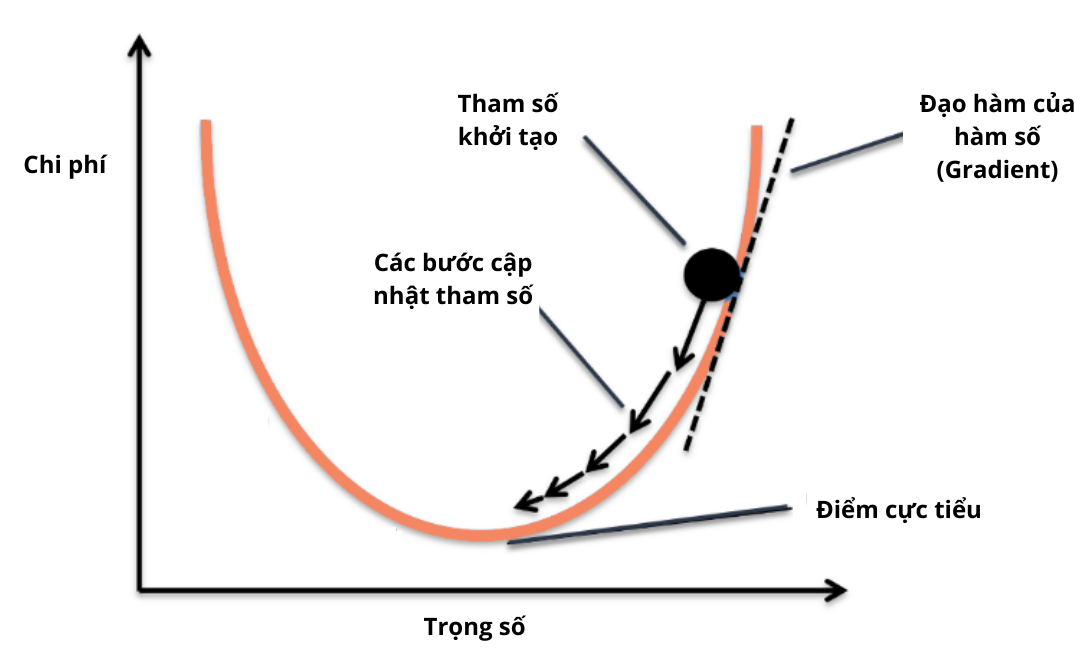
\includegraphics[width=\textwidth]{images/Chapter2/GD.png}
    \caption{Minh họa quá trình tìm điểm cực tiểu của hàm chi phi thông qua thuật toán ``Gradient descent''.}
    \label{fig:2.4_GD}
\end{figure}

Với $W = {W_0, W_1, \dots, W_k}$ là véc-tơ chứa các tham số của hàm chi phí, $k$ là số lượng các tham số; $C(W)$ là hàm chi phí của mô hình dựa trên bộ tham số $W$. Cụ thể, thuật toán ``Gradient descent'' sẽ được thực hiện bằng cách lặp lại quá trình cập nhật bộ tham số $W$ cho đến khi thỏa điều kiện dừng như sau:
\begin{equation}
    W_j = W_j - \alpha \frac{\partial C(W)}{\partial W_j}
\end{equation}
Trong đó:
\begin{itemize}
    \item $\alpha$ là siêu tham số đại diện cho learning rate của thuật toán, nó quyết định độ lớn của mỗi lần cập nhật. Khi $alpha$ nhỏ sẽ dẫn đến mỗi lần cập nhật sẽ có độ lớn nhỏ hơn và khi $alpha$ lớn thì mỗi lần cập nhật sẽ có độ lớn lớn hơn. Trong hình \ref{fig:2.4_GD} $alpha$ là độ lớn của mỗi mũi tên trong quá trình cập nhật tham số.
    \item $j \in \{0,1,\dots,k\}$ là chỉ số của các tham số trong hàm chi phí.
    \item $\frac{\partial C(W)}{\partial W_j}$ là đạo hàm riêng của hàm chi phí, nó được sử dụng để xác định hướng cập nhật của tham số. Trong hình \ref{fig:2.4_GD} đạo hàm riêng của hàm chi phí được sử dụng để xác định hướng của mũi tên trong việc cập nhật tham số.
\end{itemize}

Siêu tham số $\alpha$ là một tham số cực kì quan trọng trong thuật toán ``Gradient descent''. Vì $\alpha$ đại diện cho learning rate của thuật toán, nên khi $\alpha$ quá nhỏ thuật toán ``Gradient descent'' sẽ tốn rất nhiều thời gian trong việc đạt đến điểm cực tiểu của hàm chi phí (hội tụ). Ngược lại, khi $\alpha$ quá lớn mặc dù làm độ lớn của các tham số được cập nhật qua mỗi vòng lặp lớn hơn, tuy nhiên nó có thể dẫn đến việc các tham số cập nhật có thể bị vượt quá điểm cực tiểu, thậm chí có thể sẽ dẫn đến tình trạng thuật toán không thể đạt đến điểm cực tiểu của hàm chi phí (không thể hội tụ).